% vim: set ts=4 sw=4 tw=80 noexpandtab:
%******************************************************************************%
%                                                                              %
%                   H2SFractal.tex                                             %
%                   Made by: Kai                                               %
%                                                                              %
%******************************************************************************%

\documentclass{42-en}

%******************************************************************************%
%                                                                              %
%                                   Prologue                                   %
%                                                                              %
%******************************************************************************%

\begin{document}

\title{Graphics with Processing: Fractals!}
\subtitle{Explore the dizzyingly beautiful world of fractals and imaginary numbers}

\member {Kai}{kai@42.us.org}

\summary
{
	This assignment mirrors one that we do in the C programming language at the main 42 program. This progject is meant to create graphically beautiful fractals.
}

\maketitle

\tableofcontents


%******************************************************************************%
%                                                                              %
%                                 Inspiration                                  %
%                                                                              %
%******************************************************************************%

\chapter{Inspiration}

The term fractal was first used by mathematician Benoit Mandelbrot in 1974,
he based it on the Latin word \texttt{fractus}, meaning "broken" or "fractured".
A fractal is an abstract mathematical object, like a curve or a surface, which has a similar
pattern whatever the scale.\\

Various natural phenomena – like the romanesco cabbage, river channels, ice crystals, – have some fractal features.\\

\begin{center}
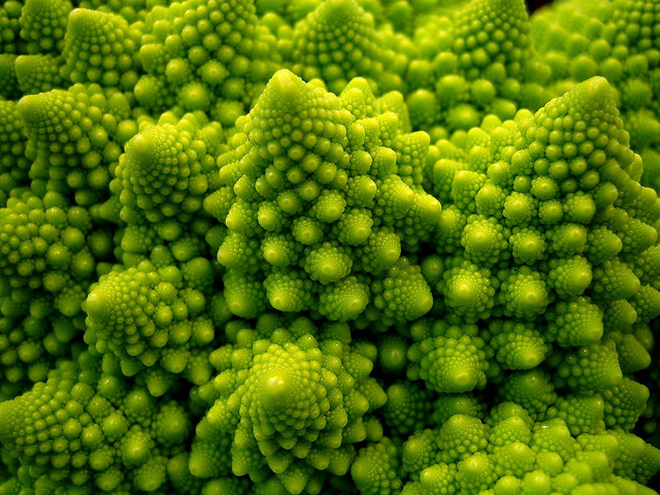
\includegraphics[width=0.6\textwidth]{romanesco.jpg}
\\
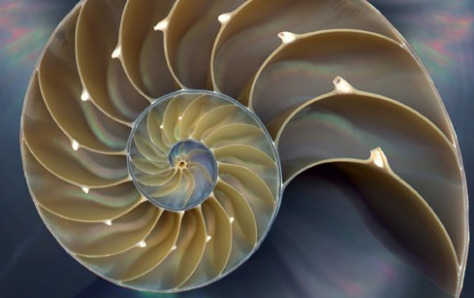
\includegraphics[width=0.6\textwidth]{fractal-nautilus.jpg}
\end{center}

%******************************************************************************%
%                                                                              %
%                                 Mathematics                                  %
%                                                                              %
%******************************************************************************%

\chapter{Mathematics}

Wikipedia discusses both the stereotypical description of a fractal (it looks the same zoomed-in as it does zoomed-out) and a more accurate mathematical description, which has to do with surface-to-volume ratio rather than aesthetics: \\

Fractals are different from other geometric figures because of the way in which they scale. Doubling the edge lengths of a polygon multiplies its area by four, which is two (the ratio of the new to the old side length) raised to the power of two (the dimension of the space the polygon resides in). Likewise, if the radius of a sphere is doubled, its volume scales by eight, which is two (the ratio of the new to the old radius) to the power of three (the dimension that the sphere resides in). But if a fractal's one-dimensional lengths are all doubled, the spatial content of the fractal scales by a power that is not necessarily an integer. This power is called the fractal dimension of the fractal, and it usually exceeds the fractal's topological dimension.\\

Wrap your brain around this visualization of it: \href{https://www.youtube.com/watch?v=gB9n2gHsHN4}{3Blue1Brown: Fractals are typically not self-similar}\\

Have you studied imaginary or complex numbers in school? Go to campus and ask your math teacher for some help - they will love that you are curious about it. :) In order to calculate classic fractals such as the Mandelbrot and the Julia set, you will need to understand how to multiply quadratic equations involving the square root of negative one, "i".\\

Now, it’s your turn to model some magnificent fractals!

%******************************************************************************%
%                                                                              %
%                                 Objectives                                   %
%                                                                              %
%******************************************************************************%

\chapter{Objectives}

You should use the PDF on the parent project to get started working with the graphics library, Processing.\\

Processing allows you to draw with shapes, or pixel by pixel. It allows you to take input from the mouse and keyboard as well to create interactive visualizations that respond to user actions.\\

We'd like you to choose your favorite fractal and create an interactive version that allows the user to zoom in, zoom out, move side to side, and change color or other parameters.


%******************************************************************************%
%                                                                              %
%                                 Mandatory                                    %
%                                                                              %
%******************************************************************************%

\chapter{Mandatory Part}

Create two different types of fractals and implement them so that we can zoom in and out, and shift them side to side or up and down. Color them beautifully and add an option to change the color scheme by pressing some key on the keyboard.\\

It's a good idea to implement the Mandelbrot as one of your first ones - it's a classic and it is mathematically related to the Julia set, which stands as your bonus.

%******************************************************************************%
%                                                                              %
%                                 Bonus                                        %
%                                                                              %
%******************************************************************************%

\chapter{Bonus Part}

Create an interactive Julia fractal in which the constant, \texttt{c}, varies by the position of the mouse in the window.

\begin{center}
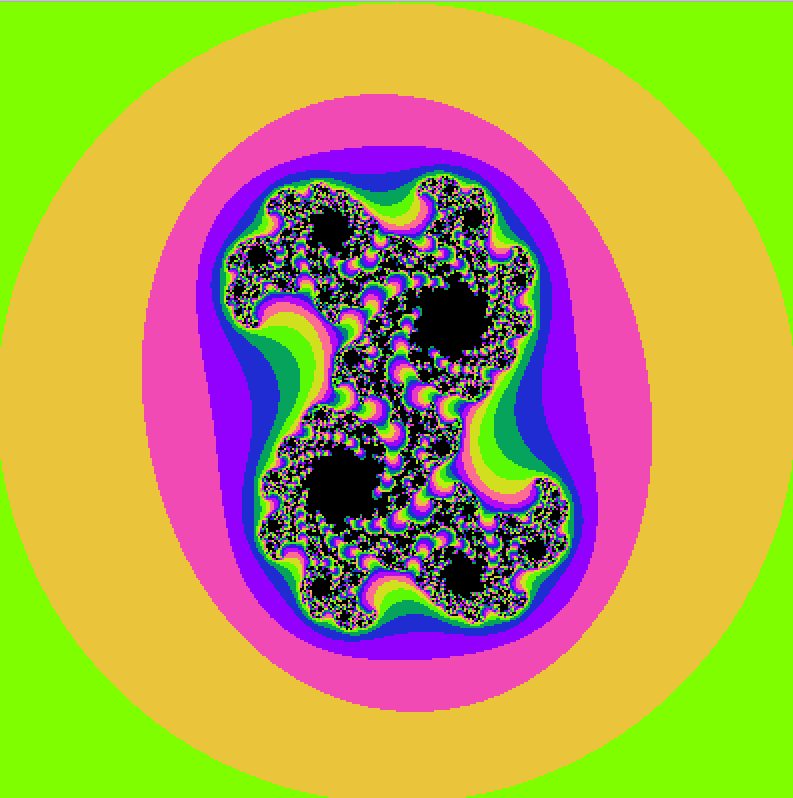
\includegraphics[width=0.6\textwidth]{julia.png}
\end{center}

\end{document}